\documentclass[10pt,a4paper]{article}
\usepackage[utf8]{inputenc}
\usepackage{amsmath}
\usepackage{amsfonts}
\usepackage{amssymb}
\usepackage{graphicx}
\usepackage{listings}
\usepackage{placeins}
\let\Oldsubsection\subsection
\renewcommand{\subsection}{\FloatBarrier\Oldsubsection}
\usepackage{color}
\definecolor{dkgreen}{rgb}{0,0.6,0}
\definecolor{gray}{rgb}{0.95,0.95,0.95}
\definecolor{darkgray}{rgb}{0.7,0.7,0.7}

\definecolor{mauve}{rgb}{0.58,0,0.82}

\lstset{frame=single,
  frameround=ffff,
  language=R,
  aboveskip=3mm,
  belowskip=3mm,
  showstringspaces=false,
  columns=flexible,
  basicstyle={\small\ttfamily},
  numbers=none,
  numberstyle=\color{mauve},
  morekeywords={1,2,3,4,5,6,7,8,9,0},
  keywordstyle=\color{blue},
  %keywordstyle=\color{blue},
  commentstyle=\color{dkgreen},
  stringstyle=\color{mauve},
  backgroundcolor=\color{gray},
  rulecolor=\color{darkgray},
  breaklines=true,
  breakatwhitespace=true,
  tabsize=3
}
\begin{document}
\section{Question 1}
\subsection{Design an R function to evaluate the
empirical ACF for a given series up to a specified maximum lag and plots it along
with a data plot.}


\begin{lstlisting}
my.acf <- function(y, lag) {
  
  N <- length(y)
  y.mean <- mean(y)
  
  out <- numeric(lag + 1)
  out[1] <- var(y)
  
  # Evaluating ACF for each lag
  for(h in 2:(lag + 1)) {
    temp <- 0.0
    for(t in 1:(N-(h-1))) {
      temp <- temp + (y[t] - y.mean) * (y[t+(h-1)] - y.mean)
    }
    out[h] <- temp/N
  }
  # Rescale to form autocorrelation function
  out <- out/out[1]
  # Plotting ACF and time series
  par(mfrow = c(2, 1))
  grid <- seq(from = 0, to = lag, len = length(out))
  plot.ts(y, type = "l", ylab = expression(Y[t]), main = "Time Series")
  plot(grid, out, type = "h", main = "ACF", xlab = "Lag", ylab = "ACF")
  # Plotting x axis
  abline(h = 0)
  # Plotting confidence intervals
  abline(h = 2/sqrt(N), lty = 2, col = "red")
  abline(h = -2/sqrt(N), lty = 2, col = "red")
  par(mfrow = c(1, 1))
  
}
\end{lstlisting}


\subsection{Take $Y_t$ = $\epsilon_t$ where $\epsilon_t$
is Gaussian white noise.}
\begin{lstlisting}
T <- 200
Y <- rnorm(T, 0, 1)
my.acf(Y)
\end{lstlisting}


\begin{figure}[ht]
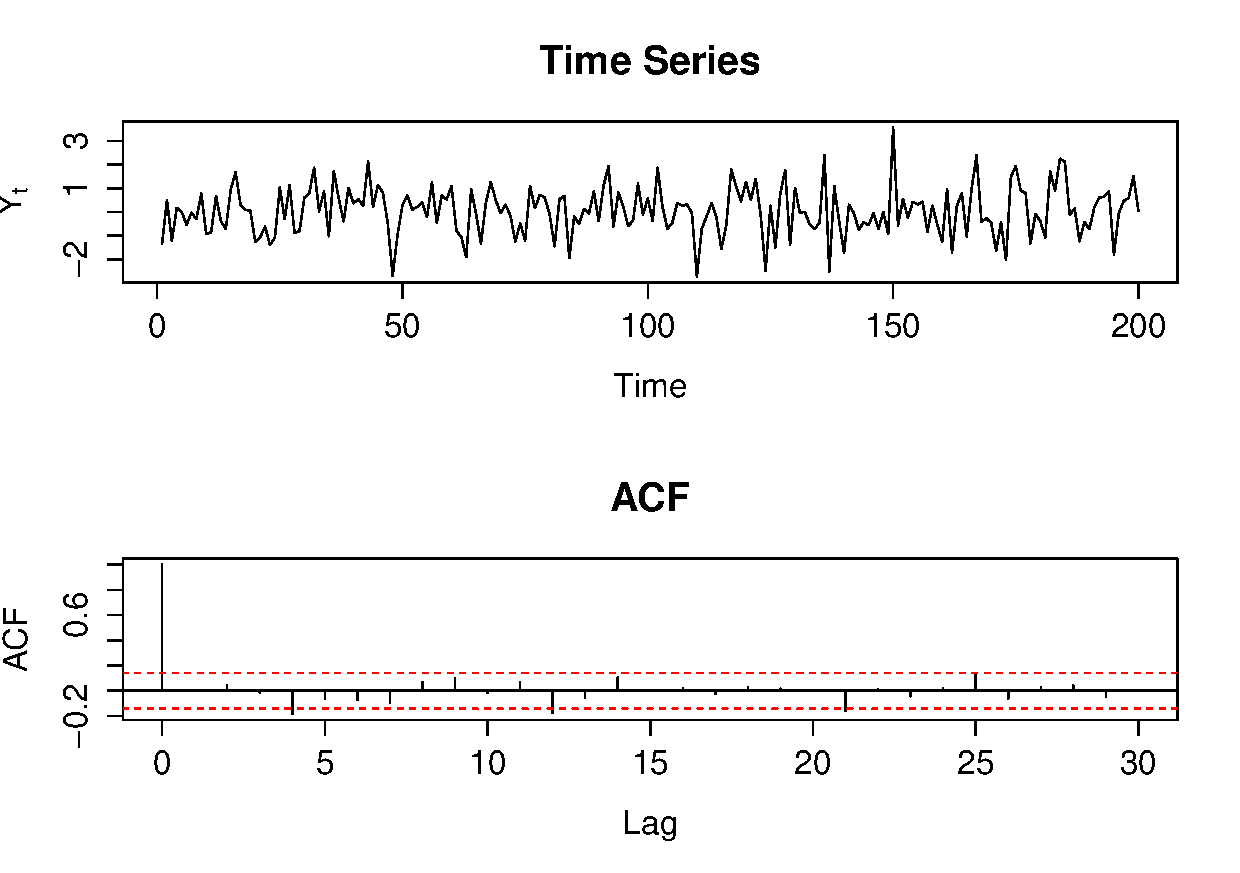
\includegraphics[width=\linewidth]{plots/p2.pdf}
\caption{Time series and ACF plot for series where $Y_t = \epsilon_t$ showing no significant autocorrelation at any lag $>0$}
\end{figure}

As the time series is drawn from an $iid$ process, we observe that the autocorrelation is not found to be significant at any lag, $0, \dots, 30$.

\subsection{Take $Y_t$ to be white noise with outliers. Generate a white noise process as in P2 and randomly choose a number of time points at which you simulate from a Gaussian
distribution with a much larger variance. Identify how the ACF deviates from that
in P2 and relate these differences to the form of the simulated series.}

\begin{lstlisting}
T <- 200
Y.outliers <- rnorm(T, 0, 1)

# Percentege of outliers
n.outliers <- 20
outliers.indexes <- sample(T, n.outliers)

# Simulating outliers from normal (0, 10)
Y.outliers[outliers.indexes] <- replicate(n.outliers, rnorm(1, 0, 20))

par(mfrow = c(2, 1))  
plot(Y)
plot(Y.outliers)
par(mfrow = c(1, 1))

#ACF
acf(Y)
acf(Y.outliers)
\end{lstlisting}
\begin{figure}[ht]
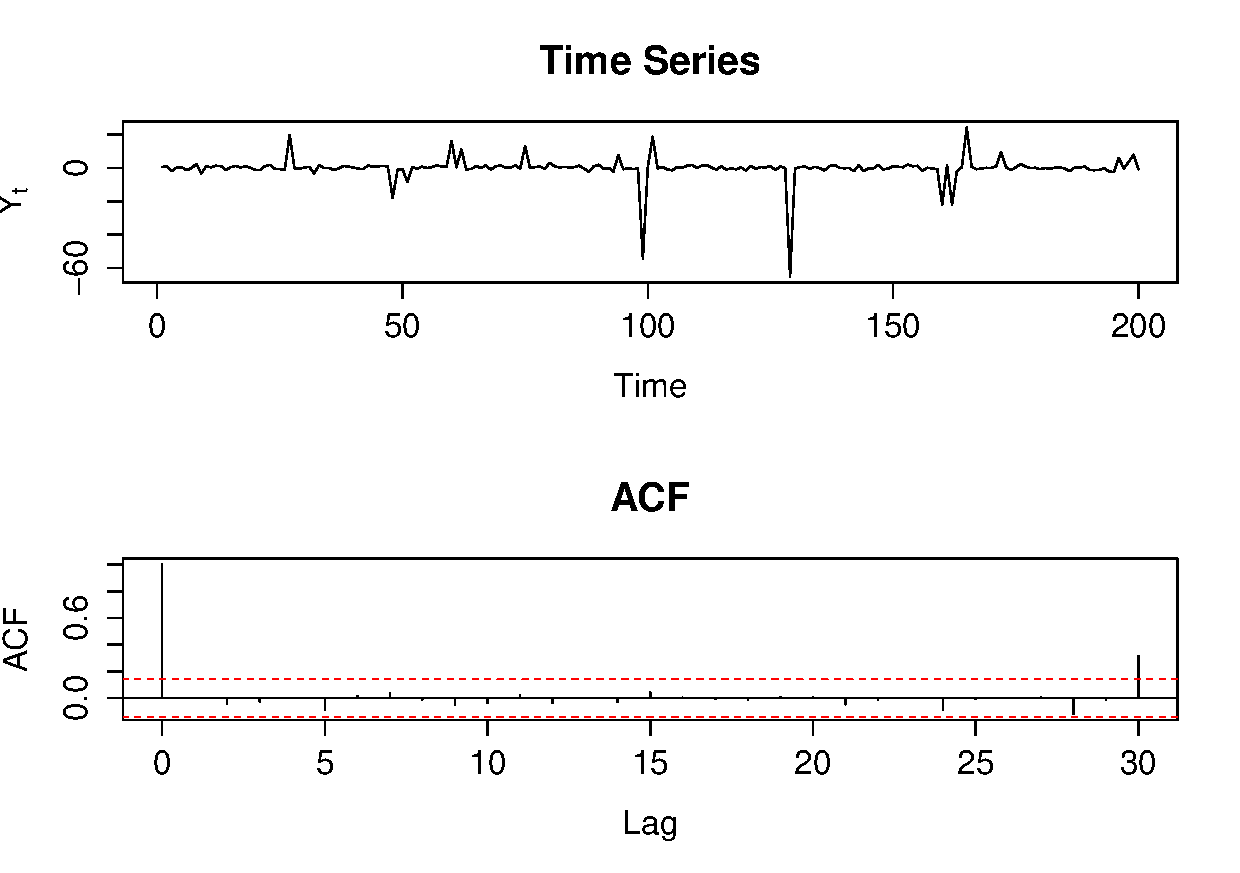
\includegraphics[width=\linewidth]{plots/p3.pdf}
\caption{Time series and ACF plot for series where $Y_t = \epsilon_t$ with random observations simulated with larger variance. The ACF plot shows a significant autocorrelation at lag 30.}
\end{figure}

Assuming the outliers are truly anomalous within the data they can adversely affect our understanding of the process. The ACF shows a significant autocorrelation at lag 30 in the data, when we know these data were generated from white noise with outliers.


\subsection{Take $Y_t$ to be a Normal Random walk: 
$Y_t = Y_{t-1} + \epsilon_t$ and $Y_1 = \epsilon_1$}
\begin{lstlisting}
T <- 200
random.walk <- numeric(T)
errors <- rnorm(T, 0, 1)

random.walk <- errors[1]
for(t in 2:T) {
  random.walk[t] <- random.walk[t-1] + errors[t]
}

my.acf(random.walk, lag = 30)
\end{lstlisting}
\begin{figure}[ht]
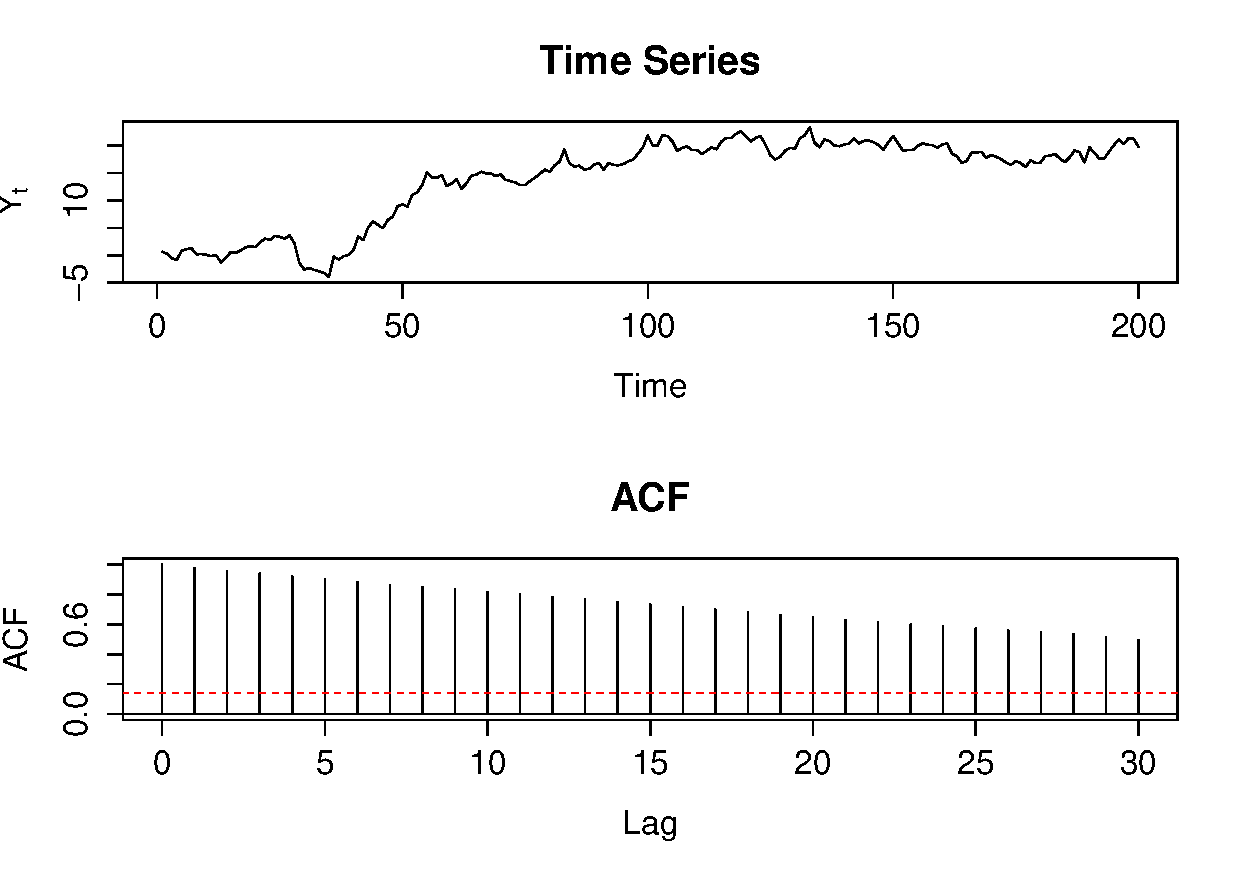
\includegraphics[width=\linewidth]{plots/p4.pdf}
\caption{Time series and ACF plot for random walk.}
\end{figure}

The autocorrelation in a random walk process decays slowly as expected as observations are strongly related to previous observations.

\subsection{Take $Y_t$ to be an autoregressive process of order 1, AR(1):
$Y_t = \alpha Y_{t-1} + \epsilon_t$ where $|\alpha| < 1$. \\
When simulating the series take $Y_1$ to be sample from the unconditional or stationary
distribution of the AR(1) process, namely
$Y_t \sim N\left(0, \frac{\sigma_e^2}{1 - \alpha^2}\right)$
where $\sigma_e^2 = Var(\epsilon_t)$.\\
Determine the effect of $\alpha$ on the behaviour of the series and its ACF. Derive the true ACF of the AR(1) process and compare with your plots of
empirical ACF. \\
Verify that the estimated ACF converges towards the true ACF as
N is increased.}

As $\alpha$ approaches $1$ we see the process devolves to a random walk process (Figure 7).

\begin{lstlisting}
ar1 <- function(alpha, T = 200) {
  errors <- rnorm(T)
  Y <- numeric(T)
  Y[1] <- rnorm(1, 0, sd = sqrt((1/(1-alpha^2))))
  for(t in 2:T) {
    Y[t] <- alpha * Y[t-1] + errors[t]
  }
  Y
}
\end{lstlisting}

\begin{lstlisting}
my.acf(ar1(alpha = 0, T = 200), lag = 30)
my.acf(ar1(alpha = 0.5, T = 200), lag = 30)
my.acf(ar1(alpha = -0.5, T = 200), lag = 30)
my.acf(ar1(alpha = 0.999, T = 200), lag = 30)


acf.ar1 <- function(alpha, h) {
  (alpha^h)
}

acf(ar1(alpha = -0.8, T = 200))
lines(x = 0:30 + 0.5, y = acf.ar1(alpha = -0.8, 0:30), type = "h", lty = 2, col = "red")

acf(ar1(alpha = -0.8, T = 1e5))
lines(x = 0:30 + 0.5, y = acf.ar1(alpha = -0.8, 0:30), type = "h", lty = 2, col = "red")

\end{lstlisting}

\begin{figure}[h!]
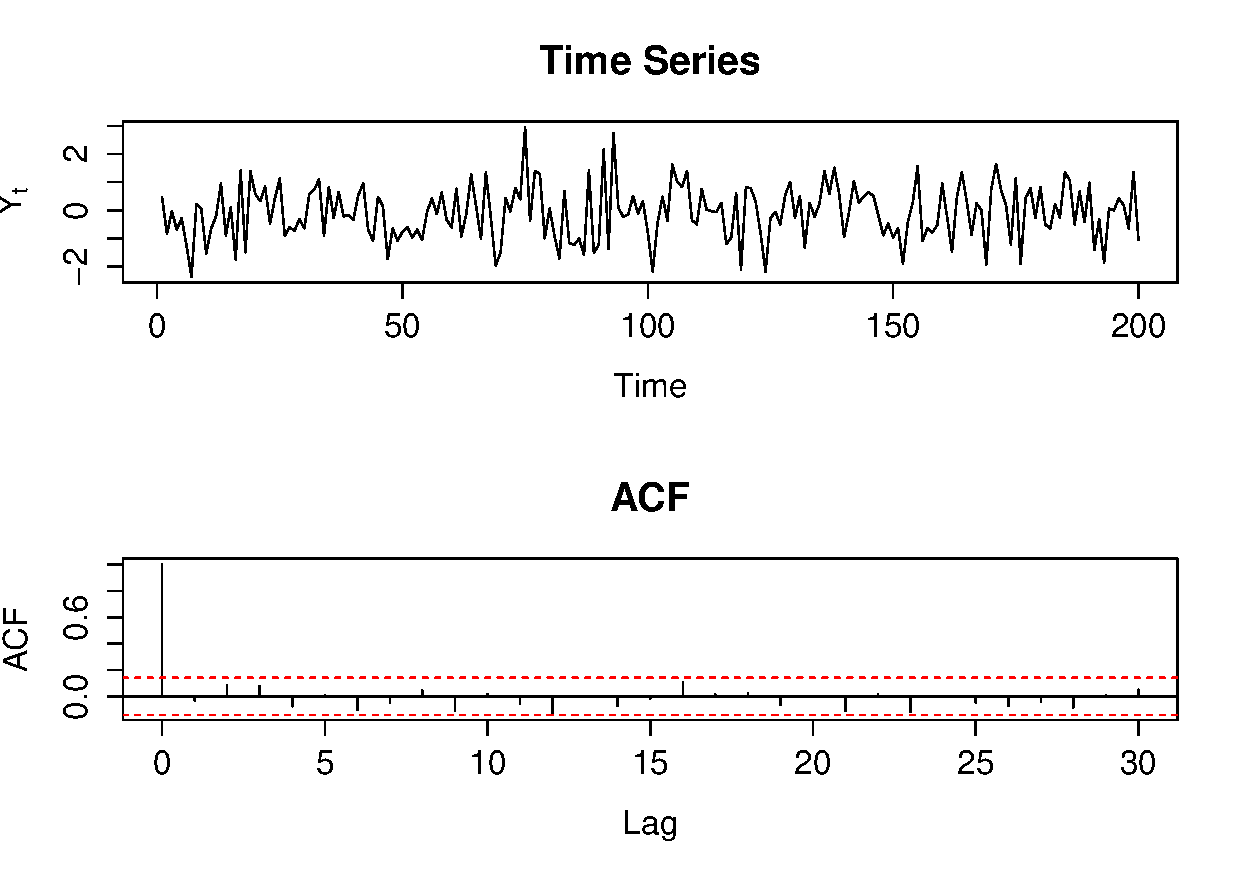
\includegraphics[width=\linewidth]{plots/p5_alpha0.pdf}
\caption{Time series and ACF plot for AR(1) with $\alpha = 0$.}
\end{figure}


\begin{figure}[h!]
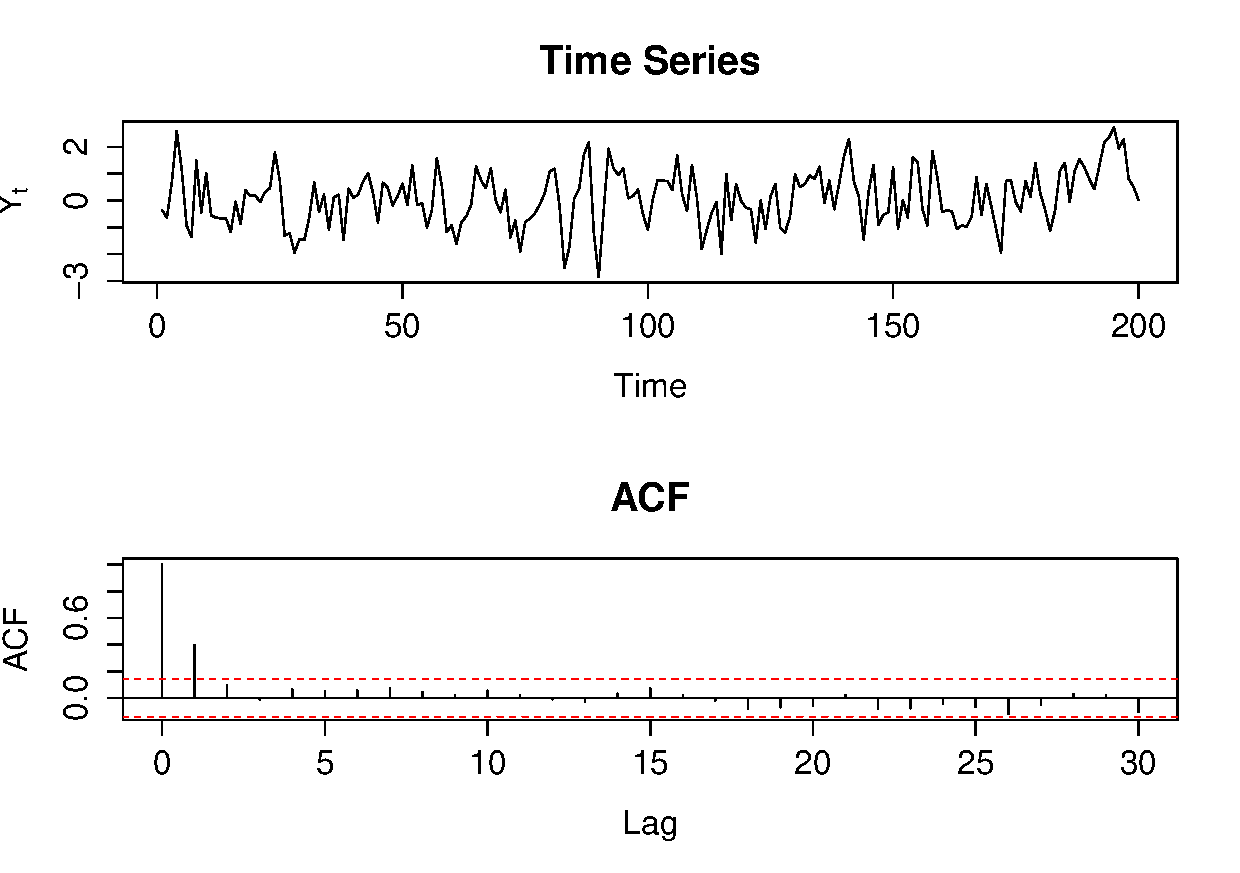
\includegraphics[width=\linewidth]{plots/p5_alpha05.pdf}
\caption{Time series and ACF plot for AR(1) with $\alpha = 0.5$.}
\end{figure}


\begin{figure}[h!]
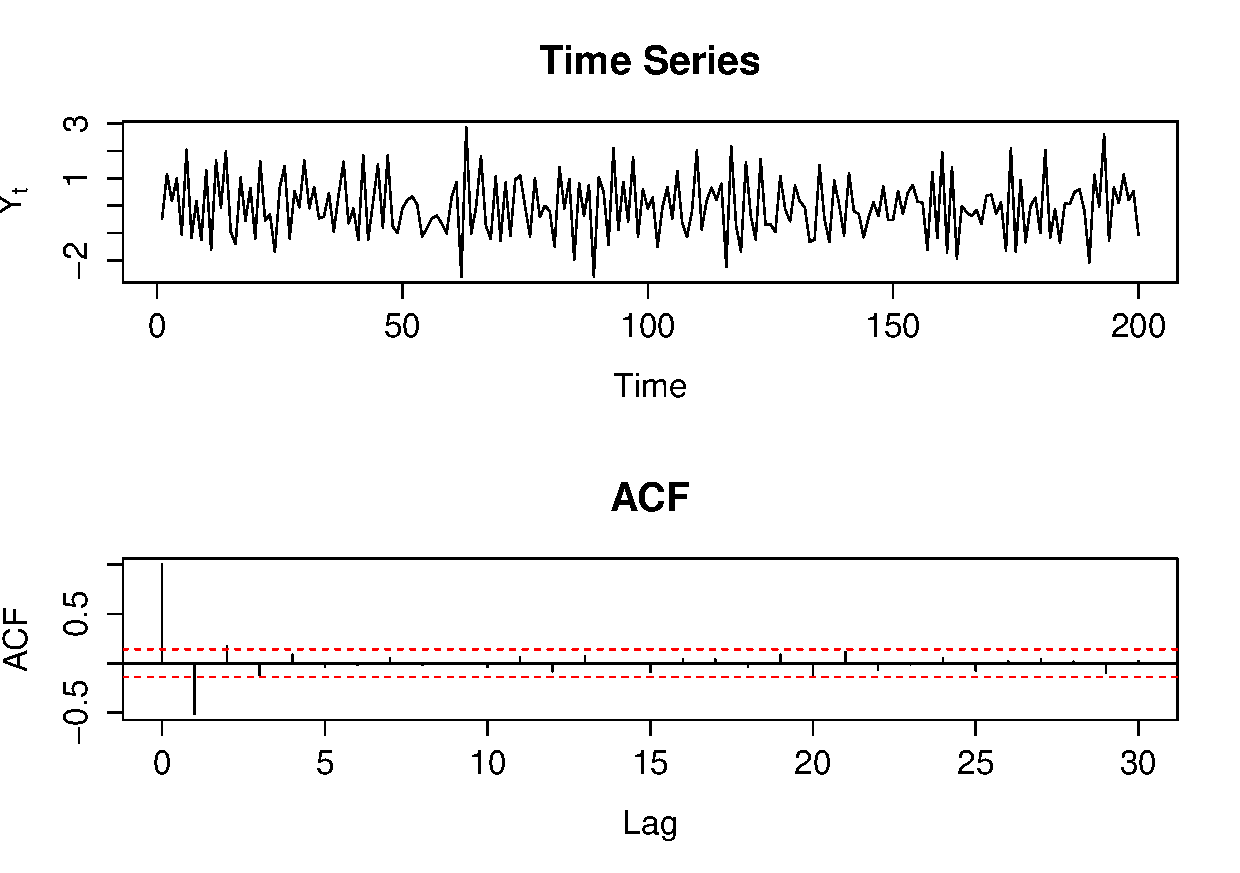
\includegraphics[width=\linewidth]{plots/p5_alphaneg05.pdf}
\caption{Time series and ACF plot for AR(1) with $\alpha = -0.5$.}
\end{figure}


\begin{figure}[h!]
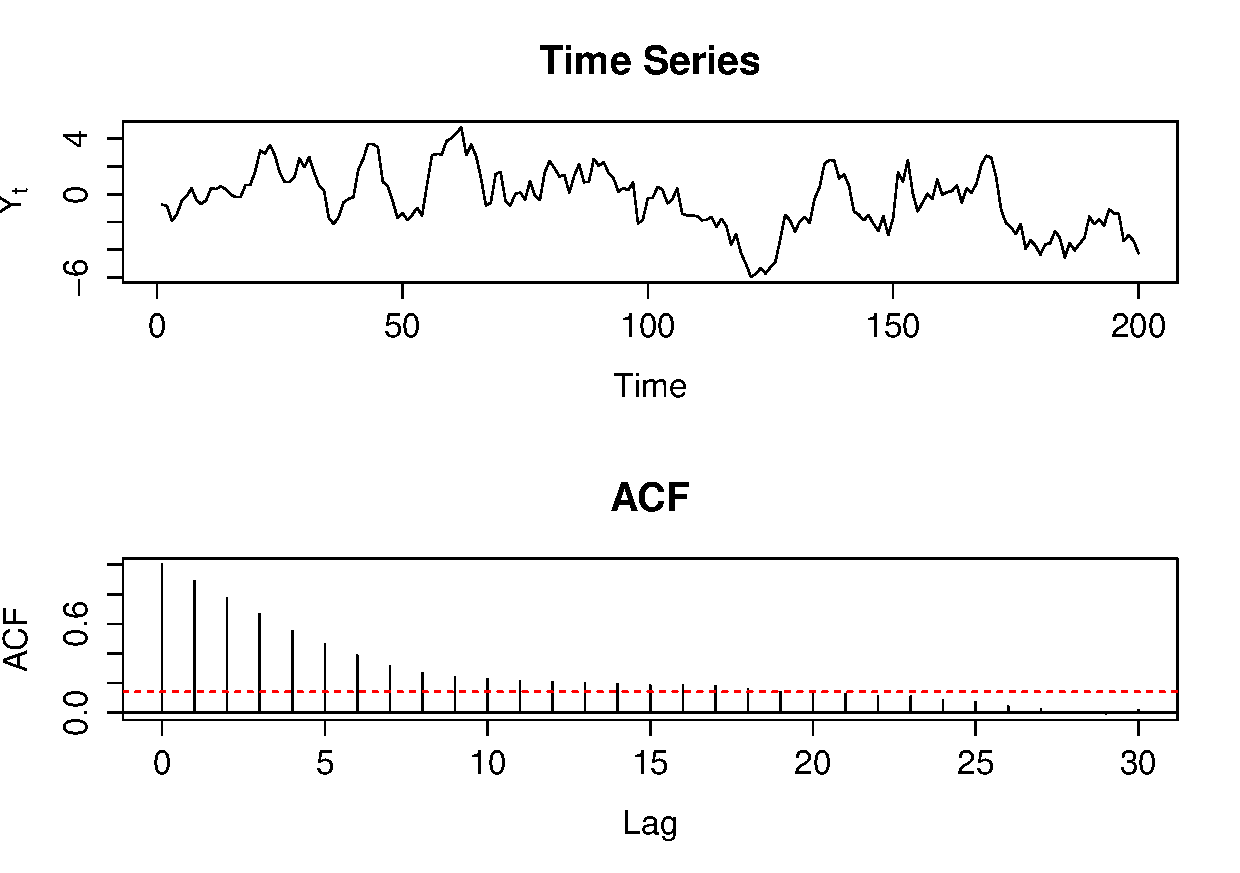
\includegraphics[width=\linewidth]{plots/p5_alpha1.pdf}
\caption{Time series and ACF plot for AR(1) with $\alpha = 0.999$.}
\end{figure}


\begin{figure}[h!]
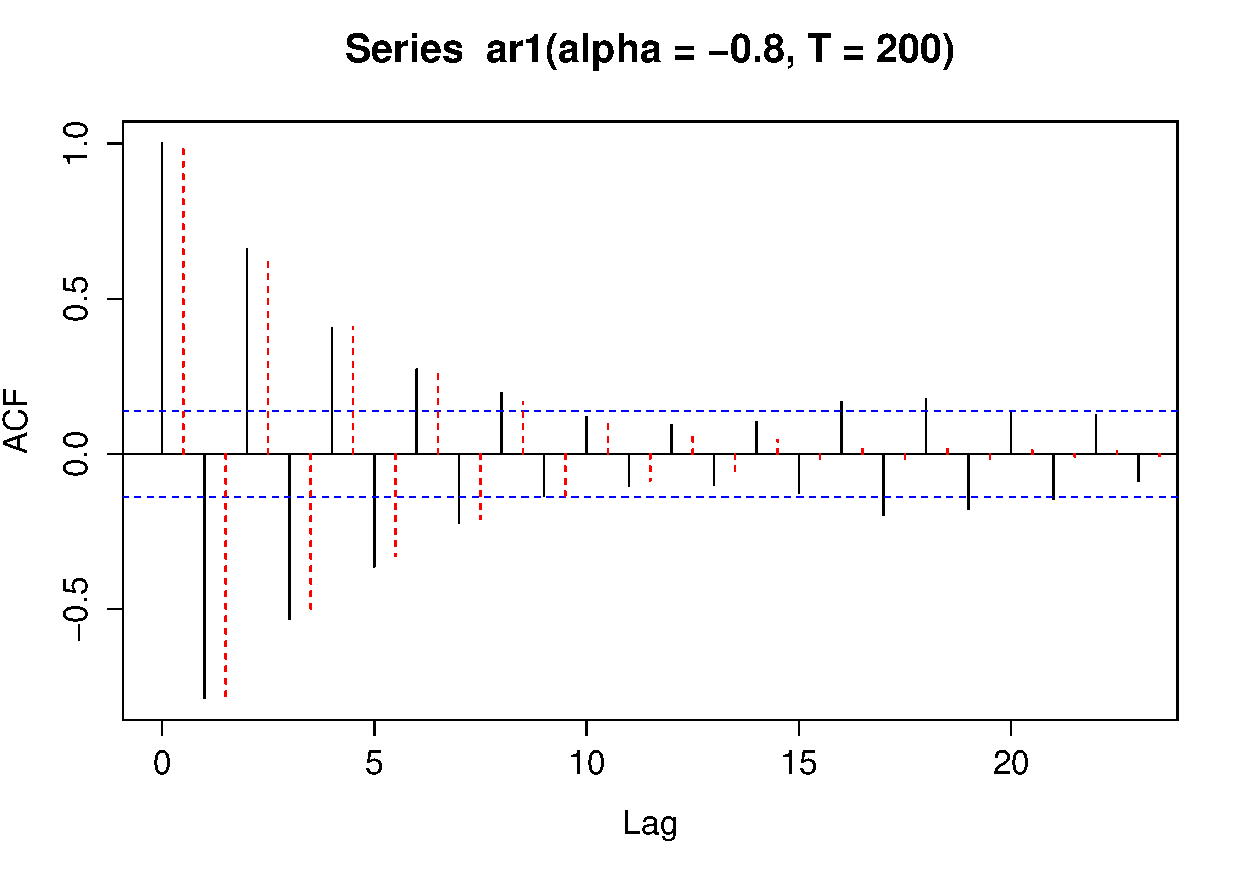
\includegraphics[width=\linewidth]{plots/p5_empacf.pdf}
\caption{The empirical (solid) and true (dashed) ACF for a time series of length $200$.}
\end{figure}
\begin{figure}[h!]
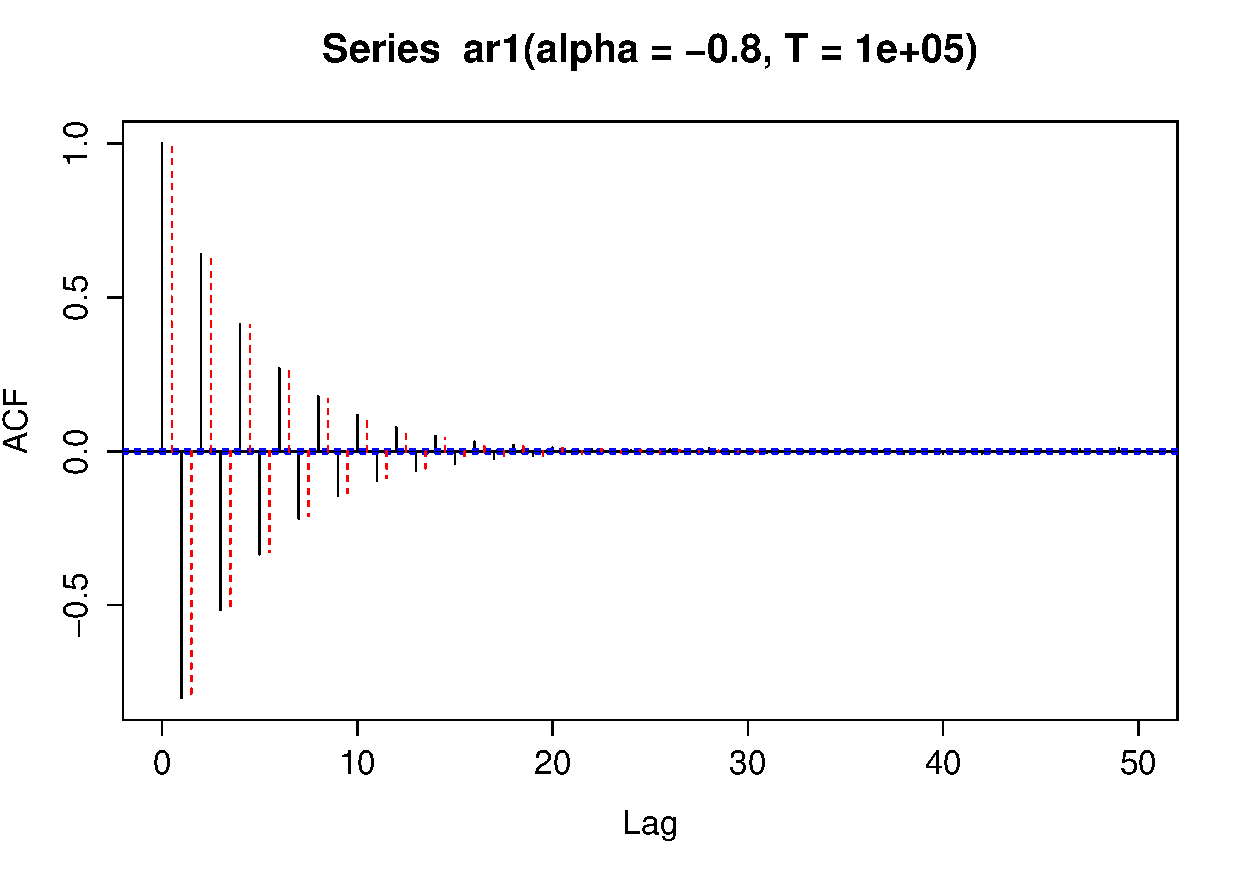
\includegraphics[width=\linewidth]{plots/p5_trueacf.pdf}
\caption{The empirical (solid) and true (dashed) ACF for a time series of length $100,000$.}
\end{figure}



\subsection{Take $Y_t$ to be the deterministic logistic process defined by \\
$Y_T = \lambda Y_{t-1}(1 - Y_{t-1})$ \\
where $Y_1 \epsilon (0, 1)$ and $0 < \lambda \leq 4$ \\
}
\begin{lstlisting}
T <- 200
Y <- numeric(T)
Y[1] <- runif(1)
lambda <- 0.5

for(t in 2:T) {
  Y[t] <- lambda*Y[t-1]*(1 - Y[t-1])
}

my.acf(Y, 30)
\end{lstlisting}


\subsection{Write a function to generate an AR(2) process for given $r_1$ and $r_2$ (write $\alpha_1$ and $\alpha_2$ as functions of $r_1$, $r_2$). Although it
is possible to simulate $Y_1$ and $Y_2$ directly from the unconditional distribution it is
simpler to first generate an AR(2) process from arbitrary starting values and then
take $Y_1$ and $Y_2$ from the end of this series.
Let $R_1 = 1/r_1$ and $R_2 = 1/r_2$. The true ACF of the AR(2) process for $h \geq 0$ is \\
$\rho(h) = \left(\frac{R_1}{1-R_1^2} - \frac{R_2}{1-R_2^2}\right)^{-1}\left(\frac{R_1^{h+1}}{1-R_1^2} - \frac{R_2^{h+1}}{1-R_2^2}\right)$ \\
Examine the effect of $r_1$ and $r_2$ on the autocorrelation structure of the AR(2) process.
}

\begin{lstlisting}
ar2_sim <- function(r1, r2, len = 200) {
  out <- rep(0, len)
  a1 <- (1 / r1) + (1 / r2)
  a2 <- - 1 / (r1 * r2)
  out <- arima.sim(n = len, list(ar = c(a1, a2)))
  out
}

true_acf <- function(r1, r2, h) {
  R1 <- 1 / r1
  R2 <- 1 / r2
  rho <- ((R1 / (1 - R1 ^ 2) - R2 / (1 - R2 ^ 2)) ^ - 1) * 
         ((R1 ^ (h + 1)) / (1 - R1 ^ 2) - ((R2 ^ (h + 1)) / (1 - R2 ^ 2)))
  rho
}
\end{lstlisting}

\begin{figure}[h!]
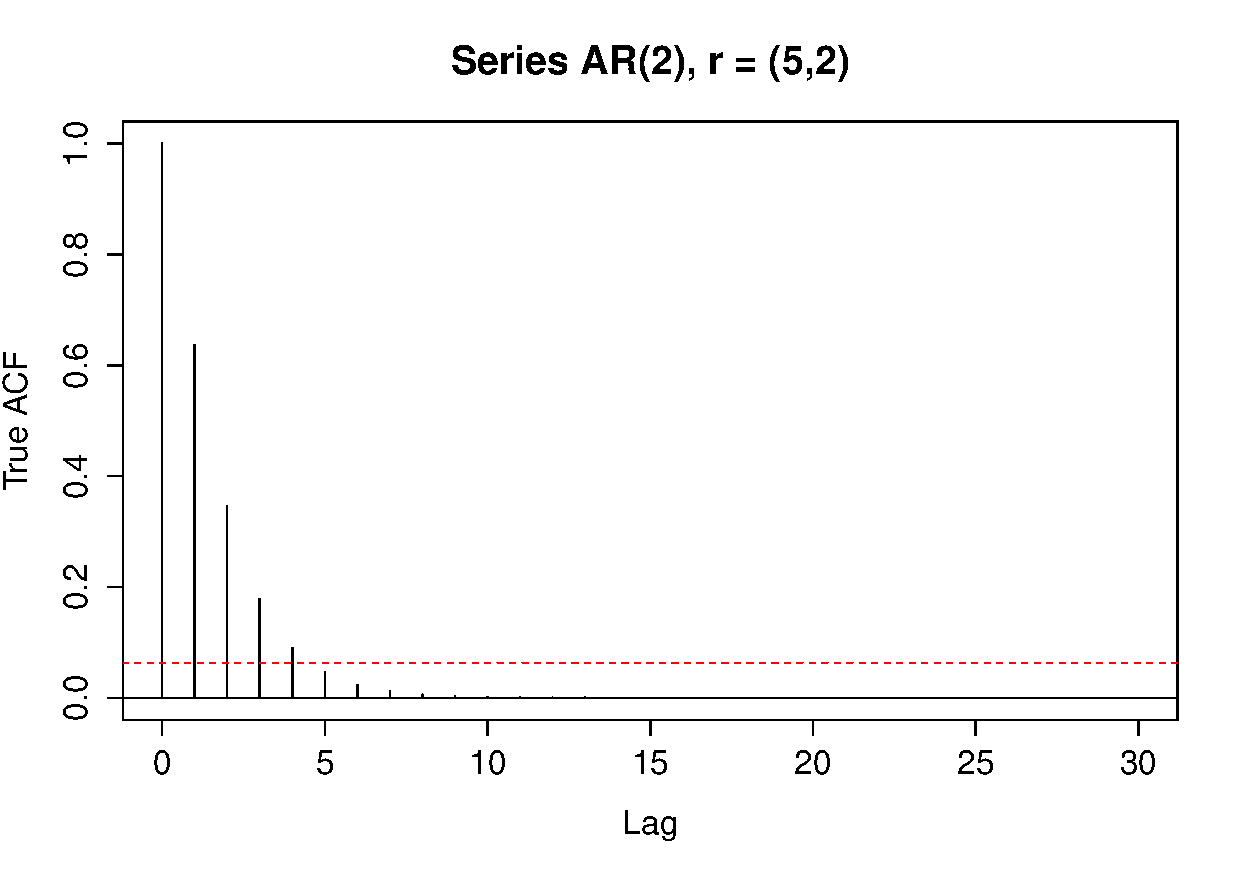
\includegraphics[width=\linewidth]{plots/p7_5_2.pdf}
\caption{Time series and ACF plot for $r=(5, 2)$.}
\end{figure}

\begin{figure}[h!]
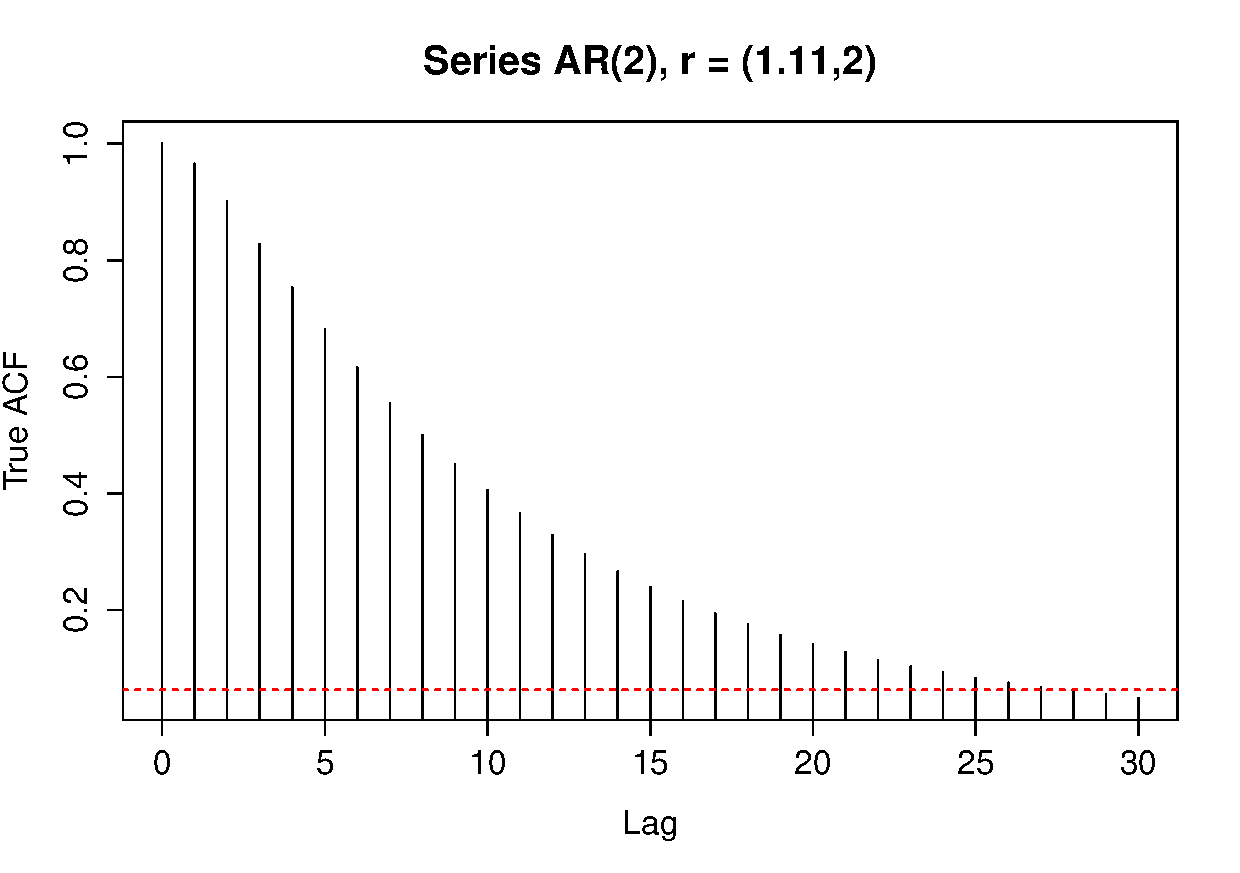
\includegraphics[width=\linewidth]{plots/p7_1_2.pdf}
\caption{Time series and ACF plot for $r=(10/9, 2)$.}
\end{figure}

\begin{figure}[h!]
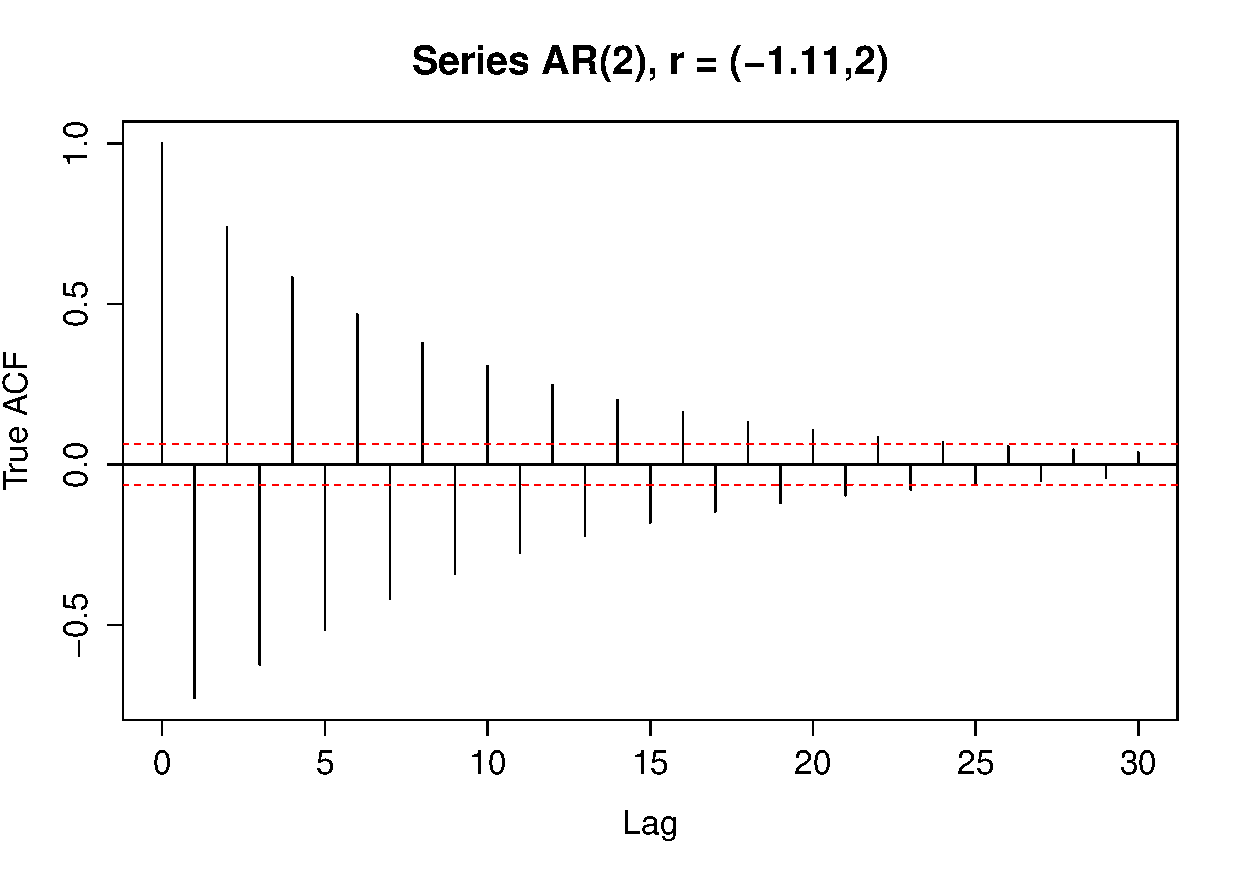
\includegraphics[width=\linewidth]{plots/p7_neg_1_2.pdf}
\caption{Time series and ACF plot for $r=(-10/9, 2)$.}
\end{figure}

\begin{figure}[h!]
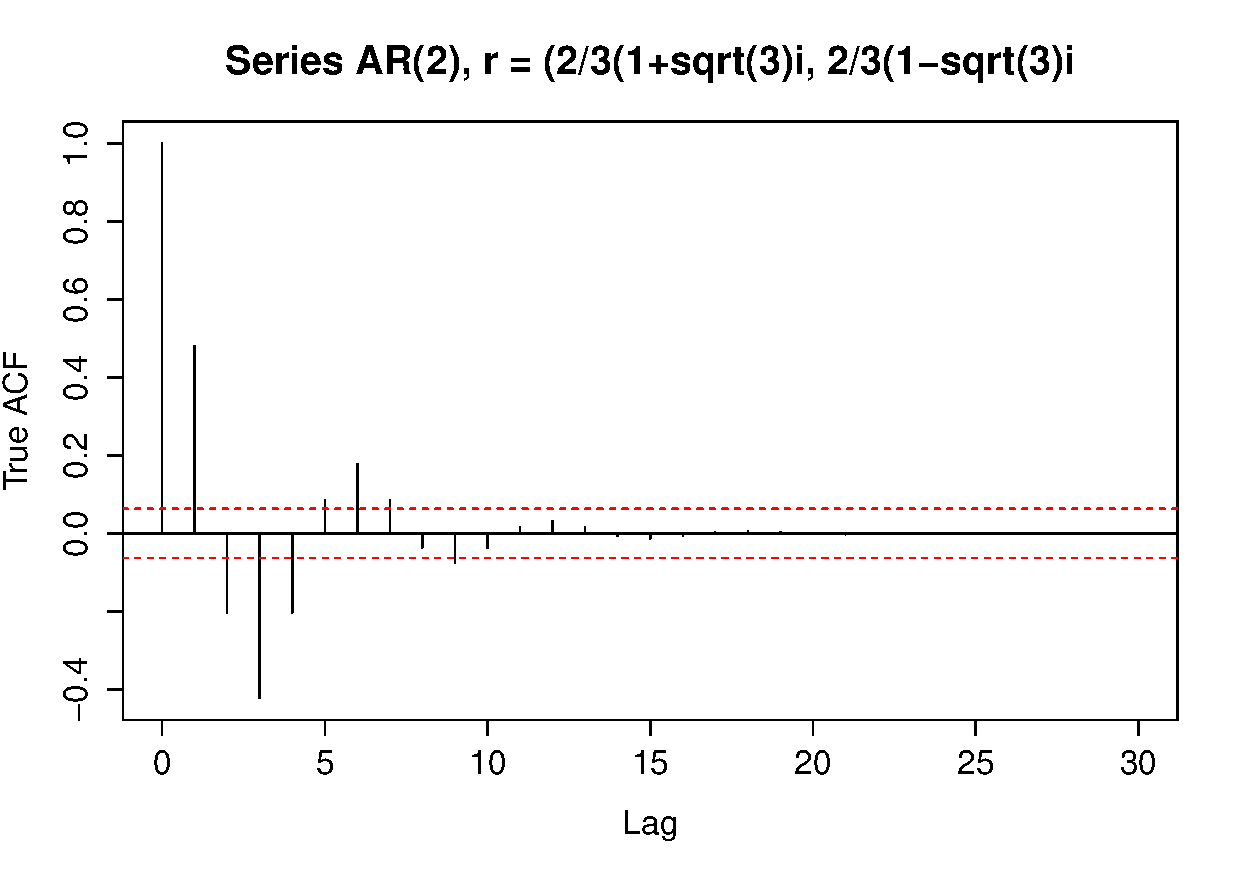
\includegraphics[width=\linewidth]{plots/p7_img_1.pdf}
\caption{Time series and ACF plot for $r=(\frac{2}{3}(1 \pm\sqrt{3}i))$.}
\end{figure}

\begin{figure}[h!]
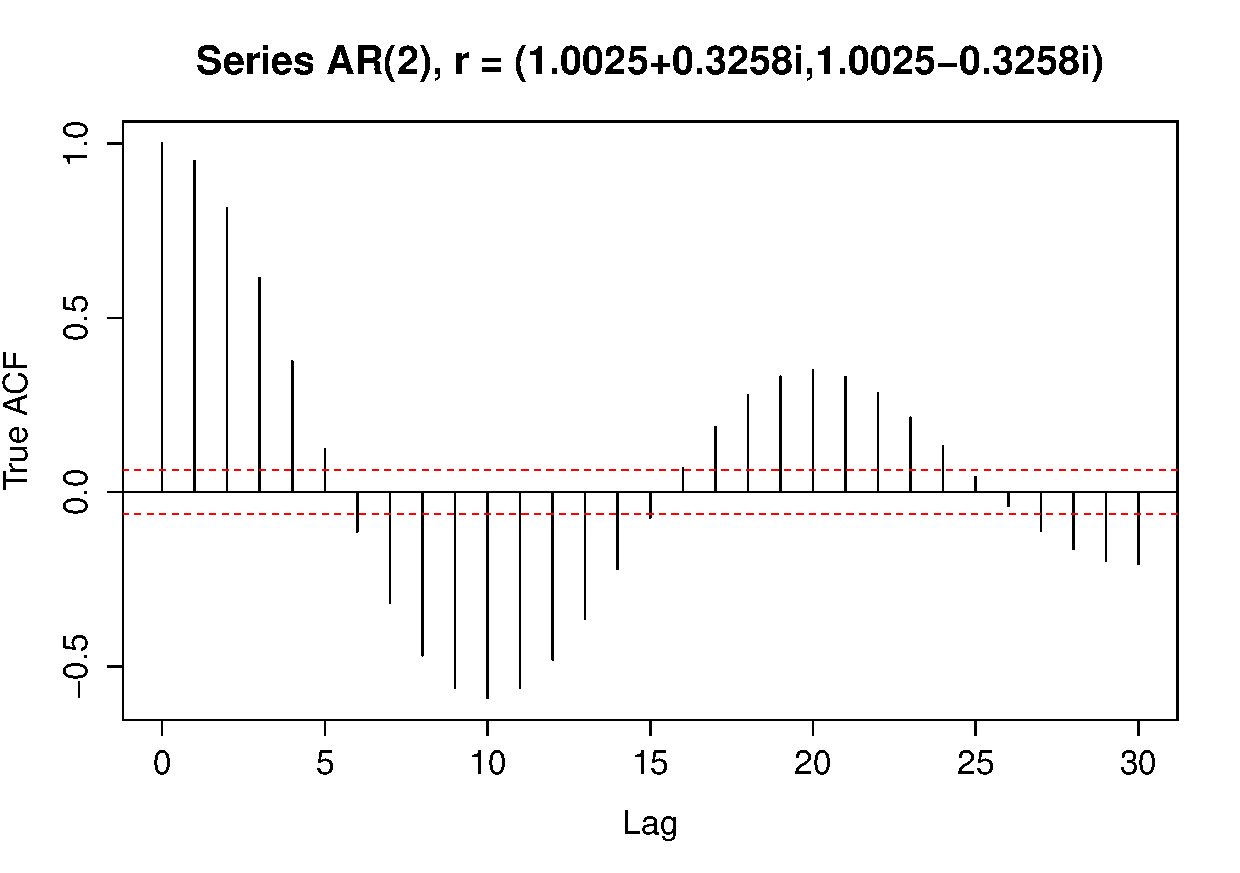
\includegraphics[width=\linewidth]{plots/p7_img_2.pdf}
\caption{Time series and ACF plot for $r=(1.0025 \pm0.3258i))$.}
\end{figure}


\end{document}